\chapter{Introduction}
\label{chap:introduction}

\section{Motivation}
The last few decades have seen the most pronounced technology evolution in history, in many different research areas and consumer markets: from robotics to smartphones, from medicine to cars, etc. One of the pillars upon which all these advancements have been made possible is the Internet, or more generally the entire set of networking technologies that allow software to communicate. 


The process towards interconnected devices saw a big leap forward in the early 1960s with the first research into packet switching as an alternative to the old circuit switching. But it is 1982 the year of standardization for the TCP/IP protocol suite, which permitted the expansion of interconnected networks  [wiki]. The Internet grew rapidly, passing from a few tens of million users in the 1990s to almost 3 billions users in 2014 [\href{http://www.internetlivestats.com/internet-users}{ref}]. Even more astonishing is the number of networked devices and connections globally, around 14 billion in 2014 [\href{http://www.cisco.com/c/en/us/solutions/service-provider/visual-networking-index-vni/index.html#~complete-forecast}{ref}].

\begin{figure}[!htb]
\centering
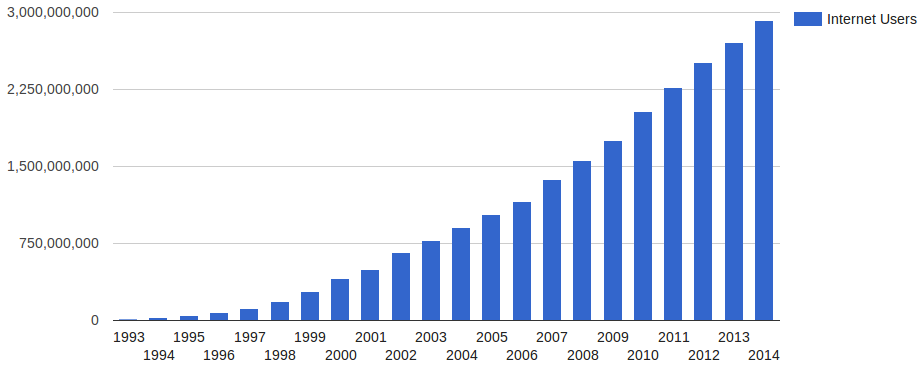
\includegraphics[width=\textwidth]{images/internet_growth}
\caption{The expansion of the Internet}
\label{fig:internet_growth}
\end{figure}

"Networks" is a very generic term. In the IT context, a computer network is set of connected nodes adopting common protocols to exchange data. The most widespread protocol for networking communication is the above-mentioned TCP/IP protocol, that is used in the vast majority of services like the World Wide Web, email, file transfer, remote system access, etc. It is also often used as a communication protocol in private networks and datacenters.
The reason for its wide adoption is not because there aren't good alternatives: TCP/IP is not to most performing protocol in every network environment, but it is fairly simple and it introduces a relatively low complexity in the overall architecture, still guaranteeing all the basic security and reliability requirements. Back in the 1980s, TCP/IP was the simpler way for applications to use most networks, and eventually it was chosen as the protocol used in the Internet, thus quickly becoming a de-facto standard [\href{http://www.computerworld.com/article/2593612/networking/tcp-ip.html}{ref}]. 
During its life, the TCP/IP protocol suite have seen updates and additional components to reach the desired levels of network congestion, traffic load balancing, handling of unpredictable behaviors, security, user-experience and so on. Such aspects became more and more challenging with the uncontrollable expansion of the Internet. 


Albeit, after all these years the core components of the TCP/IP protocol design haven't changed at all, mainly for retro-compatibility reasons. This inevitably causes some aspects of the protocol to look very limited in the current networking reality. A striking example is the scarcity of available IPv4 addresses: when TCP/IP was designed in the early stages, a 32-bit number seemed to be a very high number to encompass all the users of the network. Nevertheless, due to the unexpected increase rate in the number of Internet users (and also due to inefficient IP allocation policies), the available IPv4 addresses run out quickly, forcing the introduction of the lengthy 126-bit address format, known as IPv6, formalized in 1998. IPv6 is intended to replace IPv4, but the transition to the new format turned out to be a remarkably complicated procedure overall: IPv6 is not designed to be directly interoperable with IPv4, and even if nowadays the majority of the systems are IPv6-compatible, it took about 20 years to reach the current percentage of overall adoption: 10\% [percentage of IPv6 users accessing Google \href{http://www.google.com/intl/en/ipv6/statistics.html#tab=ipv6-adoption&tab=ipv6-adoption}{ref}]. This should give an idea of the big challenge that is modifying the core design aspects of the TCP/IP architecture, a recurrent topic in this paper.

\vspace{5mm}
When the TCP protocol was first developed in the 1970s, it was certainly difficult to predict the rate of growth of the networks all around the globe, not only in terms of the number of nodes involved, but also in terms of the quantity and type of the transmitted data, the increasing need of low latency for new streaming applications, the advancement in the hardware adopted to carry the data and the computing power of the interconnected devices. Today we can count billions of interconnected devices, and we have just started the era of the IoT (Internet of Things) which aims at giving communication capabilities to virtually every object commonly used in our daily life.
As a result of this process, the networks are becoming more complex and devices often use multiple interfaces to stay connected. 


Common appliances like smartphones provide both cellular connectivity and Wi-Fi modules (figure \ref{fig:smartphones}); same technologies can be often found in tablets; laptops have at least Wi-Fi capabilities plus an Ethernet port, and they support third-party receivers for connectivity through cellular networks. The argumentation is much more complex in the back-end infrastructures' scenario, which is rapidly evolving due to a new interest in BigData storage and analysis, as well as the flourishing of wide-scale low-latency streaming services (video streaming, VOIP, multiplayer videogames, etc.). Datacenters often count thousands of interconnected nodes and content-delivery servers that are capable of handling a huge number of network interfaces simultaneously.

\begin{figure}[!htb]
\centering
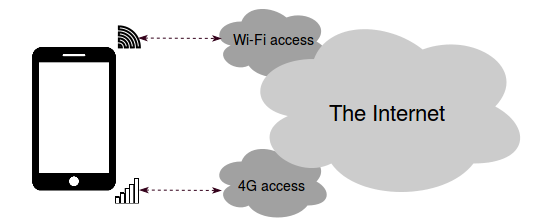
\includegraphics[width=0.75\textwidth]{images/smartphones}
\caption{The smartphone connectivity}
\label{fig:smartphones}
\end{figure}

The implications of this new reality include the possibility of establishing multiple paths to transmit data between two applications running on the communicating hosts, since they are now often equipped with multiple network interfaces, each configured with an active IP address. Back in 1970s TCP was designed to create a virtual connection between exactly two IP addresses and two port values, with almost no flexibility or dynamism in address/port addition and/or removal within the duration of the connection. In the multipath reality of the infrastructures of today, to old point-to-point singlepath connection provided by TCP looks quite limiting. This led to various projects aiming at exploiting the multipath concept, and Multipath TCP is one of them.


Multipath TCP (MPTCP) is an ongoing project managed by the Internet Engineering Task Force (IETF), whose specifications have been published as Experimental standard in January 2013 [ref RFC 6824]; such protocol extends the current TCP to introduce multipathing capabilities, maintaining retro-compatibility at the end-points and undertaking major endeavor to avoid disrupting of middleboxes' behavior. MPTPC can communicate with the application layer via standard TCP interface and it automatically splits data at the sender, it sends the data through different subflows according to the IP-addresses/interfaces available at the hosts and finally reassembles the data at the receiver, in fact enabling multipathing.

\subsection{Benefits of MPTCP}
Multipathing provides hosts with the resource pooling concept applied to networking access. Resource pooling allows dynamism and flexibility in requesting and handling resources and it is a positive trend in many services and architectures, like Content Delivery Networks (CDNs), Peer-to-Peer (P2P) networks, Cloud Computing, etc. The very concept of packet-switching, the core aspect of the modern Internet, is based on a resource pooling technique: circuit utilization is no more performed by allocating isolated channels in the link (static multiplexing) as it was the case with circuit switching, but the traffic is fragmented into small addressed packets that can share the overall link capacity (statistical multiplexing) [\href{https://www.cl.cam.ac.uk/~as2330/docs/multipath-survey.pdf}{ref}]. MPTCP aims at taking this concept to the next level, by grouping a set of separate links into a pool of links. The benefits include better resource utilization, better throughput and smoother reaction to failures, leading to an overall improved user experience, as shown in the following four major use-cases:
\begin{itemize}
  \item Combining MPTCP multipath and multihoming (the connection to the Internet via multiple providers), it is possible to achieve higher throughput by exploiting multiple simultaneous connections to transfer different portions of the same piece of data. For example, a typical smartphone could use its cellular module and its Wi-Fi module simultaneously in downloading a file from a remote server, despite them having two different IP addresses;
  \item It is possible to introduce failure handover for the connection with no special mechanism at network or link layer. If one of the interfaces goes down or the flow of data gets interrupted for any reasons, data transfer can seamlessly continue through other interfaces;
  \item By assigning different priorities to the various flows, it would be possible to better handle data transfer through the different interfaces; this could be useful if some connectivity modules drain more battery than others, or if any interfaces are associated to a limited-capacity data-plan. For example, consider the case of a file download on a smartphone via 4G connectivity: it would be advantageous to seamlessly switch the whole data transfer to the Wi-Fi interface if that becomes available in the middle of the download, starting from the point left by the cellular connection and without the need to restart the session;
  \item Providing multipath awareness to current network stacks could improve load balancing and exploitation of the network resources in datacenters; this is a valuable aspect, considering that the network performance in datacenters is usually critical for maintaining low latency of the overall system. A similar concept applies to load balancing in ISPs' network backbones.
\end{itemize}

\subsection{Multipathing Solutions}
\vspace{5mm}
MPTCP aims at achieving all the benefits mentioned in the previous paragraph by operating at the transport layer of the traditional Internet architecture (figure \ref{fig:OSI}).

\begin{figure}[!htb]
\centering
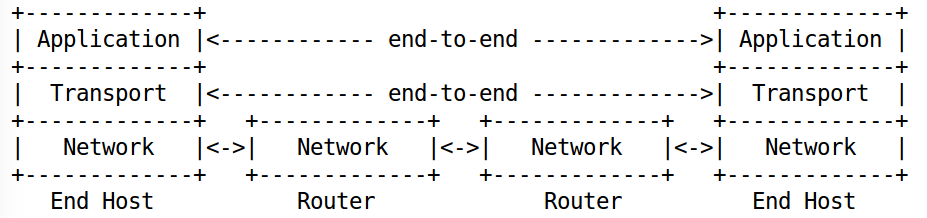
\includegraphics[width=0.75\textwidth]{images/OSI}
\caption{The traditional Internet architecture}
\label{fig:OSI}
\end{figure}

Before MPTCP, other proposals have been elaborated to achieve multipath benefits by introducing new technologies at the link layer, network layer and transport layer (the latter being the layer on which TCP operates). Even at the application layer developers can create custom frameworks on top of TCP to achieve benefits similar to those that would come by exploiting multipath natively at the lower layers. For example, most modern browsers open many TCP connection simultaneously to download the various elements of a Web Page to improve user experience. Another example could be Skype and similar VOIP services, which try to automatically reconnect hosts in case of problems with minimum impact on the user experience. Albeit all the solutions at the application layer are just clever workarounds on top of regular TCP and they fall only marginally in our discussion regarding multipath.

The following list gives a general overview of the most important multipathing solutions other than MPTCP, grouped according to the architectural layer they operate in:
\begin{itemize}
  \item \textit{Link layer}: there are link aggregation techniques to combine the capacities of different interfaces to the same switch [add a ref]. There are different ways to achieve resource pooling through link aggregation, but the basic concept is to setup multiple interfaces with the same IP address (and usually the same MAC address) so that the link aggregation is transparent to the higher-level applications and then various algorithms can be used to redistribute the data packets to the various links. In order for this to work, proper configuration is needed at the host and at the next-hop switch. Despite being a common solution in ISPs' inner networks and datacenters to improve throughput and achieve higher network-access, end-users cannot directly take advantage of this technology.


  \item \textit{Network layer}: there exist multiple solutions to better exploit multipathing at this layer, most notably \textit{Mobile IP} and \textit{Shim6}. Without going into the details, they both provide hot-handover capabilities with no interruption of the higher-level services, with some limitations: Mobile IP requires extensive support by the underlying infrastructure and Shim6 is an IPv6 only solution. More importantly, there is a fundamental problem in confining resource pooling at the network layer: TCP operates at the transport layer but it is closely related to the network layer because it statefully inspects various properties of the underlying network paths to provide performance optimizations (this is why referring to TCP often implies taking into consideration the whole TCP/IP protocol stack): in most cases, transparent modifications at the network layer would cause TCP malfunctioning.


  \item \textit{Transport layer}: the most notable experiment in multipath exploitation prior to MPTCP is the Stream Control Transmission Protocol (SCTP). Such protocol is, in many ways, similar to MPTCP: the first version of SCTP provided fail-over capabilities by exploiting different interfaces, and successive versions introduced multi-streaming capabilities to increase throughput. The major problem with SCTP is that it was thought to be an alternative, enhanced version of TCP, and the two protocol are indeed incompatible with each other. This means that a wide adoption of SCTP would require to upgrade the network to be SCTP aware. Moreover, all the applications would need to be upgraded to explicitly switch to the new protocol for communication. The vast global networking scenario of today, mainly based on TCP, makes these requirements virtually impossible to meet, and SCTP remains a technology of very limited adoption.
\end{itemize}



\vspace{5mm}
All these previous solutions didn't get widespread adoption. Link layers and network layers solutions require extensive modifications in the underlying network configurations in order to achieve the desired results; introducing a new multipath-aware protocol at the transport layer requires to change all the applications in order for them to communicate over the new protocol, thus allowing this solution in very limited scenarios; workarounds at the application layer, despite being quite effective, are far from the purpose of MPTCP.


MPTCP primary goal is to automatically introduce the multipath benefits to infrastructures and devices currently adopting TCP, with the minimum possible effort from users, developers, network maintainers. Engineers decided that the best way to achieve all these requirements was to still make use of TCP as fundamental block for communication, extending it to support multipath: the entire protocol design works by adding MPTCP custom options into regular TCP packets and each subflow in MPTCP is indeed seen by the lower infrastructure as a regular TCP connection. 

\vspace{5mm}
MPTCP got a lot of attention in the Internet community in the last few years, and many consider MPTCP as a valuable step forward for the whole global network currently relying on TCP.
The final goal of MPTCP is to replace the majority of the current TCP implementations, which is a very delicate process in which all the current TCP standards in terms of robustness and security have to be maintained, if not improved. This paper is an evaluation of the security aspects of MPTCP, with an analysis of current threats and vulnerabilities affecting the protocol.

\section{Problem Statement}
MPTCP is a big effort from the IETF working group to unlock multipath networking capabilities worldwide, with many subtle implications for current infrastructures. Hence the importance of evaluating the current security status of MPTCP, by inspecting its implications on external middleboxes and security equipment and also by analyzing internal design flaws that might allow attacks to the MPTCP sessions. The main focus of this paper is on the latter case. The main vulnerability currently known for the protocol, related to the ADD\_ADDR component, is tested and studied; the solution for it is implemented and evaluated. In the process, patches for the Linux kernel implementation of the protocol have been developed to fix the vulnerability. 


A comprehensive list of all the objectives for the thesis work is the following:
\begin{itemize}
    \item Studying the security implications of adopting MPTCP on current infrastructures; 
    \item Listing the known vulnerabilities affecting the current version of the protocol; 
    \item Studying and exploiting the ADD\_ADDR vulnerability of the protocol;
    \item Evaluating the possible solutions for the ADD\_ADDR vulnerability; 
    \item Assessing the best solution for the ADD\_ADDR vulnerability and developing it for the Linux kernel implementation of MPTCP;
    \item Developing effective and powerful simulation scenarios in order to test MPTCP (and possibly other networking protocols);
    \item Contributing to the upstreaming of MPTCP into the Linux kernel by developing patches and contributing to official RFC documentation.
\end{itemize}

\section{Methodology}
The thesis work has been carried out at the Intel Corporation offices in Lund (Sweden). The process took 6 months in total, with a main focus on testing and developing. The entire work has been closely followed by major stakeholders in the MPTCP community, located in Sweden, Romania and the United States. Such cooperation involved patch reviewing and weekly meetings.


The workflow started with an overall study of MPTCP and how it interacts with the most common middleboxes. The next step was a more focused evaluation of the current threats for the protocol, mainly referencing to the document RFC 7430; within the document, only one vulnerability is considered a blocking issue in the advancement of MPTCP standardization, known as the ADD\_ADDR vulnerability. The document also proposes a change in the protocol design that fixes the problem. With such background, the actual development stage of the work started.

\vspace{5mm}
At first, it was necessary to sync with the development status by interacting with the official MPTCP mailing list for developers [\href{https://listes-2.sipr.ucl.ac.be/sympa}{ref}]; this allowed to make sure that the ADD\_ADDR solution proposed in RFC 7430 was indeed the preferred one and that nobody started developing a patch for it already.
Before starting to work on the fix, a first stage of the work involved a deeper analysis of the ADD\_ADDR vulnerability. A connection hijacking has been executed by exploiting such vulnerability in a testing environment. This allowed to better validate the criticality of the problem and it was a useful experiment to get acquainted with MPTCP. Moreover, it was a good way to setup a proper testing environment that was indeed used during the whole patch-development process that followed.
After having reproduced the attack, it followed an analysis of the MPTCP source code within the Linux kernel in order to understand how the protocol implementation works inside the TCP stack. This step was required to get the required knowledge to start developing patches. 


The entire code developed during the stage, around 400 additions, was eventually merged into the official MPTCP repository. Some additional contributions have been performed in order to improve RFC documentation about the protocol and to upgrade related networking tools to be compatible with the new version of MPTCP.
The final evaluations and the writing of the report took place in the last two months of the working period.

\subsection{Document Structure}
The structure of this paper mainly follows the workflow explained in the previous section. After the introductory first chapter, the discussion is mainly subdivided into two parts: first, an analysis about MPTCP background and working principles (chapters 2 and 3); second, a discussion about the original work on simulating and fixing the ADD\_ADDR vulnerability (chapters 4 and 5):

\begin{itemize}
  \item Chapter 2 starts with a broad explanation of the basic concepts of TCP to introduce how MPTCP has been developed on top of it. All the technical details of the new protocol can be found in this chapter. In this chapter it is also included an analysis on the MPTCP deployment status in the real world and the problematics associated in upstreaming the protocol (mainly incompatibilities with current middleboxes).
  
  \item Chapter 3 is again a background analysis on MPTCP, with a narrowed focus on its security aspects. The chapter includes a comprehensive threats analysis, with an overview of the current security issues affecting the new protocol. An entire section is dedicated to the ADD\_ADDR vulnerability. In such section all the details regarding the vulnerability are presented: how to exploit it to hijack an MPTCP connection and what are the requirements  an attacker needs to execute the attack.
  
  \item Chapter 4 is the first part that introduces the original work carried out during the thesis period. Taking as reference the theory behind the ADD\_ADDR attack explained in the previous chapter, this section explains the development of the script capable of exploiting the vulnerability in a simulated environment. The script code is explained step-by-step, as well as the entire procedure to setup the virtual machines to execute the attack. This entire chapter aims at validating the criticality of the ADD\_ADDR vulnerability and in doing so it also provide setup guidelines for a powerful simulating environment that can be useful for future MPTCP testing and development.
  
  \item Chapter 5 contains the core part of the thesis work. It starts with a theoretical evaluation of the accepted fix for the ADD\_ADDR vulnerability and goes on with its development for the Linux kernel implementation of MPTCP. All the issues encountered during the project, as well as the required side-feature that needed to be implemented for proper functioning, are reported in this chapter. The two last sections cover the remaining part of the work: the set of contributions not mentioned in the previous sections and a final evaluation of the performance of the produced patches.
  
  \item Chapter 6 is the conclusive part of the paper, where related work and proposals for future work are present, together with some final thoughts.
\end{itemize}